\subsection{JAM with a NFW Dark Matter Halo}

\paragraph{Including a NFW halo.} The dynamical modelling attempts in the previous sections suggest that J1331's inner regions have a slightly more roundish and at large radii more massive mass distribution than expected from the distribution of stars alone. A dark matter halo in addition to the stellar component could explain these findings. We therefore proceed by modelling the mass distribution with a) a stellar component, which we get from the light MGE in Table [TO DO: REF????] times a constant stellar mass-to-light ratio $\Upsilon_*$), and b) a spherical NFW dark matter component [TO DO: Navarro 1995 or 1996???], which is implemented in the JAM modelling as a fit of a 10-Gaussian MGE to the classical NFW profile
\begin{equation*}
\rho_\text{NFW}(r) \propto 1 / \frac{r}{R_\text{s,NFW}} \left( 1 + \frac{r}{R_\text{s,NFW}} \right)^2.
\end{equation*}
The NFW halo has two free parameters, the scale length $R_\text{s,NFW}$ and a parameter describing the total mass of the halo. We use $v_\text{200}$, which is the circular velocity at the radius $r_\text{200}$ within which the mean density of the halo is 200 times the cosmological [TO DO: how to express this] critical density, i.e.
\begin{eqnarray*}
M_\text{200} &=& M(<r_{200})\\
\frac{M_{200}}{ \frac 43 \pi r_{200}^3} &=& 200 \rho_\text{crit}(z=0) \\
v_\text{200} &=& \sqrt{\frac{GM_{200}}{r_\text{200}}}
\end{eqnarray*}
with $\rho_\text{crit}(z=0)=1.43 \cdot 10^{-7} M_\odot / \text{pc}^3$ in the WMAP5 cosmology by [TO DO: REF: Dunkley et al. 2009].

\paragraph{Priors.} [TO DO: REF: Dutton et al. 2010] give a relation for halo vs. stellar mass for late-type galaxies. For an Chabrier IMF stellar population they found
\begin{equation*}
y = y_0 \left( \frac{x}{x_0} \right)^\alpha \left[ \frac 12 + \frac 12 \left(\frac{x}{x_0} \right)^\gamma \right]^{(\beta - \alpha)/\gamma},
\end{equation*}
where $x= m_*$ [$M_\odot h^{-2}$] is the stellar mass, $y = \frac{\langle M_{200}\rangle}{m_*}$ and $\langle M_{200}\rangle$ [$M_\odot h^{-2}$] is the mean halo mass. The parameters for the mean and $2\sigma$ error curves for this relation are$\alpha = -0.5\pm0.15$, $\beta = 0$, $\gamma = 1.0$, $\log_{10} x_0 = 10.4$, $\log_{10} {y_0}_{-0.24}^{+0.28}$ [TO DO: REF: Dutton et al. 2010]. Using the stellar mass estimate for J1331 from \citet{SWELLSI} $m_* = (1.06 \pm 0.25) \cdot 10^{11} M_\odot$ for the Chabrier IMF estimate [TO DO: introduce somewhere], we find ${v_{200}} = (202_{-33}^{+44})_{-13}^{+12}$. The first of the two quoted errors is due to the $2\sigma$ scatter in the relation by [TO DO: REF: Dutton et al. 2010]. The second error is the propagated error due to the uncertainty in the stellar mass. We use this rough estimate for J1331's [TO DO: Continue on page 98]



[TO DO]

\begin{figure*}
\centering
\includegraphics[width=0.9\linewidth]{fig/B4_contour_plot_short.ps}
\caption{??? Preliminary crappy caption: Result of the MCMC sampling of the parameter space for a model with NFW halo and constant velocity anisotropy. Green and blue shows the priors. Grey diamonds are the models shown in next figure. ??? [TO DO: nice caption]}
\label{fig:???}
\end{figure*}

\begin{figure*}
\centering
\begin{subfigure}{\textwidth}
  \centering
  \includegraphics[width=0.8\linewidth]{fig/B4_rms_error_curves.ps}
  \caption{???}
  \label{fig:???}
\end{subfigure}
\begin{subfigure}{.5\textwidth}
  \centering
  \includegraphics[width=0.9\linewidth]{fig/B4_jam_profiles_errors_short_vcirc.ps}
  \caption{????????}
  \label{fig:???}
\end{subfigure}%
\begin{subfigure}{.5\textwidth}
  \centering
  \includegraphics[width=0.9\linewidth]{fig/B4_jam_profiles_errors_short_projmass.ps}
  \caption{???}
  \label{fig:???}
\end{subfigure}
\caption{??? Preliminary crappy caption: 12 samples from the parameter pdf found with the MCMC above for the model with NFW halo and constant velocity anisotropy. Big red dot shows the Einstein mass with a 10\% error (used in fit). ??? [TO DO: nice caption]}
\label{fig:???}
\end{figure*}



\subsubsection{Predicting the Rotation Curve at larger Radii}

[TO DO]

\begin{figure*}
\centering
\includegraphics[width=0.7\linewidth]{fig/B4_rms_rot_curves_best_model.ps}
\caption{??? Preliminary crappy caption: Model: NFW halo and constant velocity anisotropy, using the the mean / peak values of the MCMC result in the above pdf for the model parameters. Fitting one more free parameter to the rotation curve in the inner regions, predicting the rotation curve and dispersion at larger radii. Green dots are gas kinematics. ??? [TO DO: nice caption]}
\label{fig:???}
\end{figure*}
